\documentclass[../review_1.tex]{subfiles}
\graphicspath{{\subfix{../img/}}}
\begin{document}
\chapter{Technologien und Entwicklungswerkzeuge}\thispagestyle{fancy}

\section{Hardware}
Die Software hat eine Mindestanforderung an ihre zu verwendende Hardware, hierzu gehört, dass eine sehr gute CPU vorliegt, wie z.B. ein Ryzen 9 5900X. Des weiteren wird ein genügend großer Arbeitsspeicher benötigt, dass heißt ab einer Speicherkapazität von 32GB un mehr, und genügend viel Speicherplatz, dass heißt ab 200GB aufwärts. Um das System gut einsetzen zu können müssen auch genügend schnelle Netzwerkkarten vorliegen (z.B. 25GbE), welche DPDK unterstützten.

\section{Programmiersprache und Bibliotheken}
Die für die Software verwendete Programmiersprache ist C++ auf der Version 17 und wird auf dem Betriebssystem  Ubuntu entwickelt. Als Programmiereditor und IDE wird VSCodium verwendet, welches eine Community betriebene, frei lizenzierte Distribution der Microsoft IDE VSCode ist. Zur Unterstützung der Entwicklung werden zusätzliche  Erweiterungspakete für VSCodium verwendet, unter anderem Meson (1.3.0) und das C/C++ Extension Pack (1.0.0).
Es wurde die Programmiersprache C++ gewählt, da die Mitglieder dieses Projektes innerhalb ihres Studiums schon Erfahrungen mit dieser Sprache gewonnen haben, sei es in Form von Praktika oder aus eigenen Bedürfnissen.

Ein Hauptbestandteil des Projektes ist die Verwendung des \textit{Data Plane Development Kit} (kurz \textit{DPDK}), auf der LTS-Version 20.11, das aus Bibliotheken zur Beschleunigung von Paket-verarbeitungs-Workload besteht, die auf einer Vielzahl von CPU-Architekturen laufen. Es ermöglicht die Entwicklung von Hochgeschwindigkeits-Datenpaket-Netzwerkanwendungen durch Kernel Bypässe. Mit einer Reihe von Bibliotheken ist es möglich Netzwerkschnittstellen-Controller-Treiber für den Polling-Modus zu verwenden, um die Paketverarbeitung statt im Betriebssystem-Kernel auf Anwendungen im Userspace zu ermöglichen. Durch den Einsatz von DPDK kann ein höherer Paketdurchsatz erreicht werden, als mit der Linux Nativen interruptgesteuerten Verarbeitung im Kernel. Dies ist für dieses Projekt wichtig, da hohe Übertragungsraten erreicht werden sollen.
\begin{figure}[H]
    \centering
    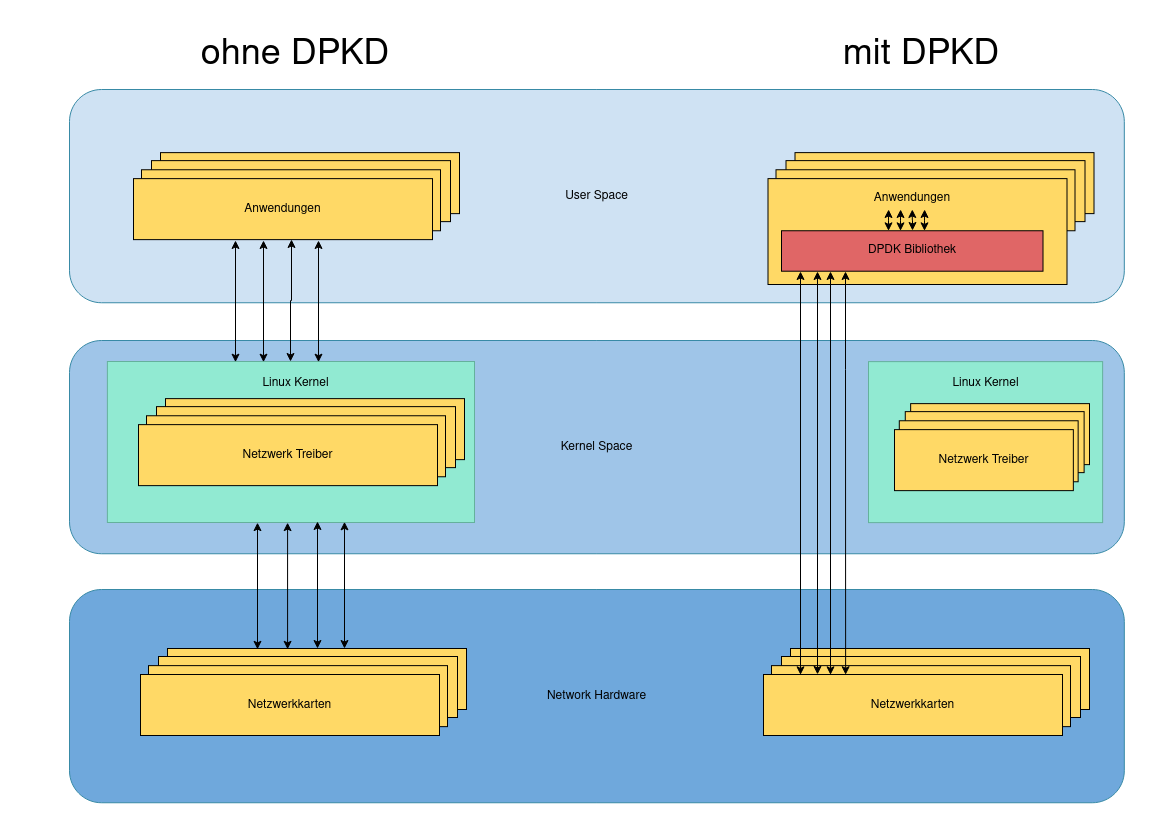
\includegraphics[width=0.7\linewidth]{mit-ohne-DPDK}
    \caption{Kernel Bypass mit DPDK gegenüber Kernel Verarbeitung}
    \label{fig:with_without_dpdk}
\end{figure}

\section{Entwicklungswerkzeuge}
Das Buildsystem wird mit Meson erstellt. Meson ist ein Open-Source-Build-System, das sowohl extrem schnell als auch benutzerfreundlich ist (im Vergleich zu CMake). Meson unterstützt viele Plattformen und nutzt Ninja für extrem schnelle vollständige und inkrementelle Builds ohne Einbußen bei der Korrektheit. Dazu gehören unterschiedliche Funktionen wie Unit-Tests, Code-Coverage-Reporting, vorkompilierte Header und dergleichen.

\section{Tools}
Für die Dokumentation wird Doxygen und Latex verwendet und für die Visualisierung von Grafiken VisualParadigm und Inkscape.

\end{document}